%%%% Proceedings format for most of ACM conferences (with the exceptions listed below) and all ICPS volumes.
\documentclass[sigconf]{acmart}
\usepackage{graphicx, wrapfig}
\graphicspath{{imgs/}}
\usepackage{lipsum}
\usepackage{stfloats}
\usepackage[english,ngerman,brazilian]{babel}
\settopmatter{printacmref=false}
\setcopyright{none}
\renewcommand\footnotetextcopyrightpermission[1]{}
\pagestyle{plain}
\captionsetup{justification   = raggedright,
              singlelinecheck = false}
\newcommand{\source}[2]{\raggedleft{}\vspace*{-7mm}\caption*{ \scriptsize{{#1}: {`#2'}}}}

\def\BibTeX{{\rm B\kern-.05em{\sc i\kern-.025em b}\kern-.08emT\kern-.1667em\lower.7ex\hbox{E}\kern-.125emX}}

% end of the preamble, start of the body of the document source.
\begin{document}

%
% The "title" command has an optional parameter, allowing the author to define a "short title" to be used in page headers.
\title[Fronteiras da Transferência de Aprendizado: uma revisão sistemática com enfoque meta-analítico]{Fronteiras da Transferência de Aprendizado: \\
uma revisão sistemática com enfoque meta-analítico}
%

\author{Fred Guth}
\email{fredguth@fredguth.com}
\affiliation{%
  \institution{Departamento de Ciência de Computação, Universidade de Brasília}
  \postcode{70.910-900}
  \city{Brasília}
  \state{DF}
  \country{Brazil}
}

\renewcommand{\shortauthors}{Guth, F.}

\begin{abstract}
  Humanos e animais conseguem aprender com poucas amostras \cite{goodfellow} e apresentam extraordinária capacidade de generalização que os algoritmos de aprendizagem de máquina ainda estão longe de alcançar. Os modelos mais bem sucedidos da atualidade exigem uma enormidade de dados bem rotulados que são caros e difíceis de obter, tornando-se hoje um dos maiores empecilhos para aplicações práticas. Tais fatos apontam para o grande potencial da área de Transferência de Aprendizado, que tem por objetivo aproveitar o conhecimento obtido em uma atividade para aprender mais eficientemente outras, que guardem alguma relação com a primeira. O presente estudo visa apresentar uma revisão sistemática da literatura e identificar, com embasamento quantitativo, as principais contribuições para a área. Além disso, usamos medidas de acoplamento bibliográfico para identificar trabalhos na fronteira do conhecimento e fizemos uma análise textual, em resumos e palavras-chave, comparando estes com os "clássicos" da área de forma a mapear para que direção a pesquisa avança.  
\end{abstract}


\begin{CCSXML}
<ccs2012>
 <concept>
 <concept_id>10010147.10010257.10010258.10010262.10010277</concept_id>
 <concept_desc>Computing methodologies~Transfer learning</concept_desc>
 <concept_significance>500</concept_significance>
 </concept>
</ccs2012>
\end{CCSXML}
\ccsdesc[500]{Computing methodologies~Transfer learning}

\keywords{transferência de aprendizado, revisão sistemática, enfoque meta-analítico}


\maketitle


\section{Introdução} 
  Em geral, o jeito padrão de se treinar um modelo de aprendizagem de máquina é sempre começar \emph{tabula rasa}, com uma inicialização aleatória dos parâmetros. Aprender assim, a partir do nada, é contrário à forma como os humanos o fazem.

  Estudos recentes~\cite{JiaLian2017, BelinkovBisk2018}, mostram que os algoritmos atuais são frágeis de forma similar aos sistemas baseado em regras: Não generalizam além de dados vistos durante o treinamento.
  \lipsum[1]
  \subsection{Contribuições}
  \lipsum[3]
  \begin{figure}[h]
    \includegraphics[width=\columnwidth]{citacoes_por_ano2.pdf}
    \source{Dados}{Web of Science (março/2019)}
    \caption{Evolução dos número de citações de artigos em Tranferência de Aprendizagem nos últimos 10 anos.}
    \label{fig:citacoes_por_ano}
  \end{figure}
  \subsection{Visão Geral e Organização do Artigo}
  \lipsum[3]
  \subsection{Trabalhos Relacionados}
  \lipsum[2]
\section{Método: Revisão Sistemática com Enfoque Meta-Analítico}
  \lipsum[1]
  \begin{itemize}
    \item{Análise de Co-citações}
    \item{Análise de Acoplamento Bibliográfico}
    \item{Análise Textual}
  \end{itemize}
  % \subsection{Sumarização}
\section{Revisão da Literatura}
  \subsection{Transferência de Aprendizagem}
  \lipsum[3]
  \subsection{Um breve histórico}
  \lipsum[2]
  \subsection{O panorama da produção científica na área}
  \lipsum[1]
    \begin{figure}[h]
    \fbox{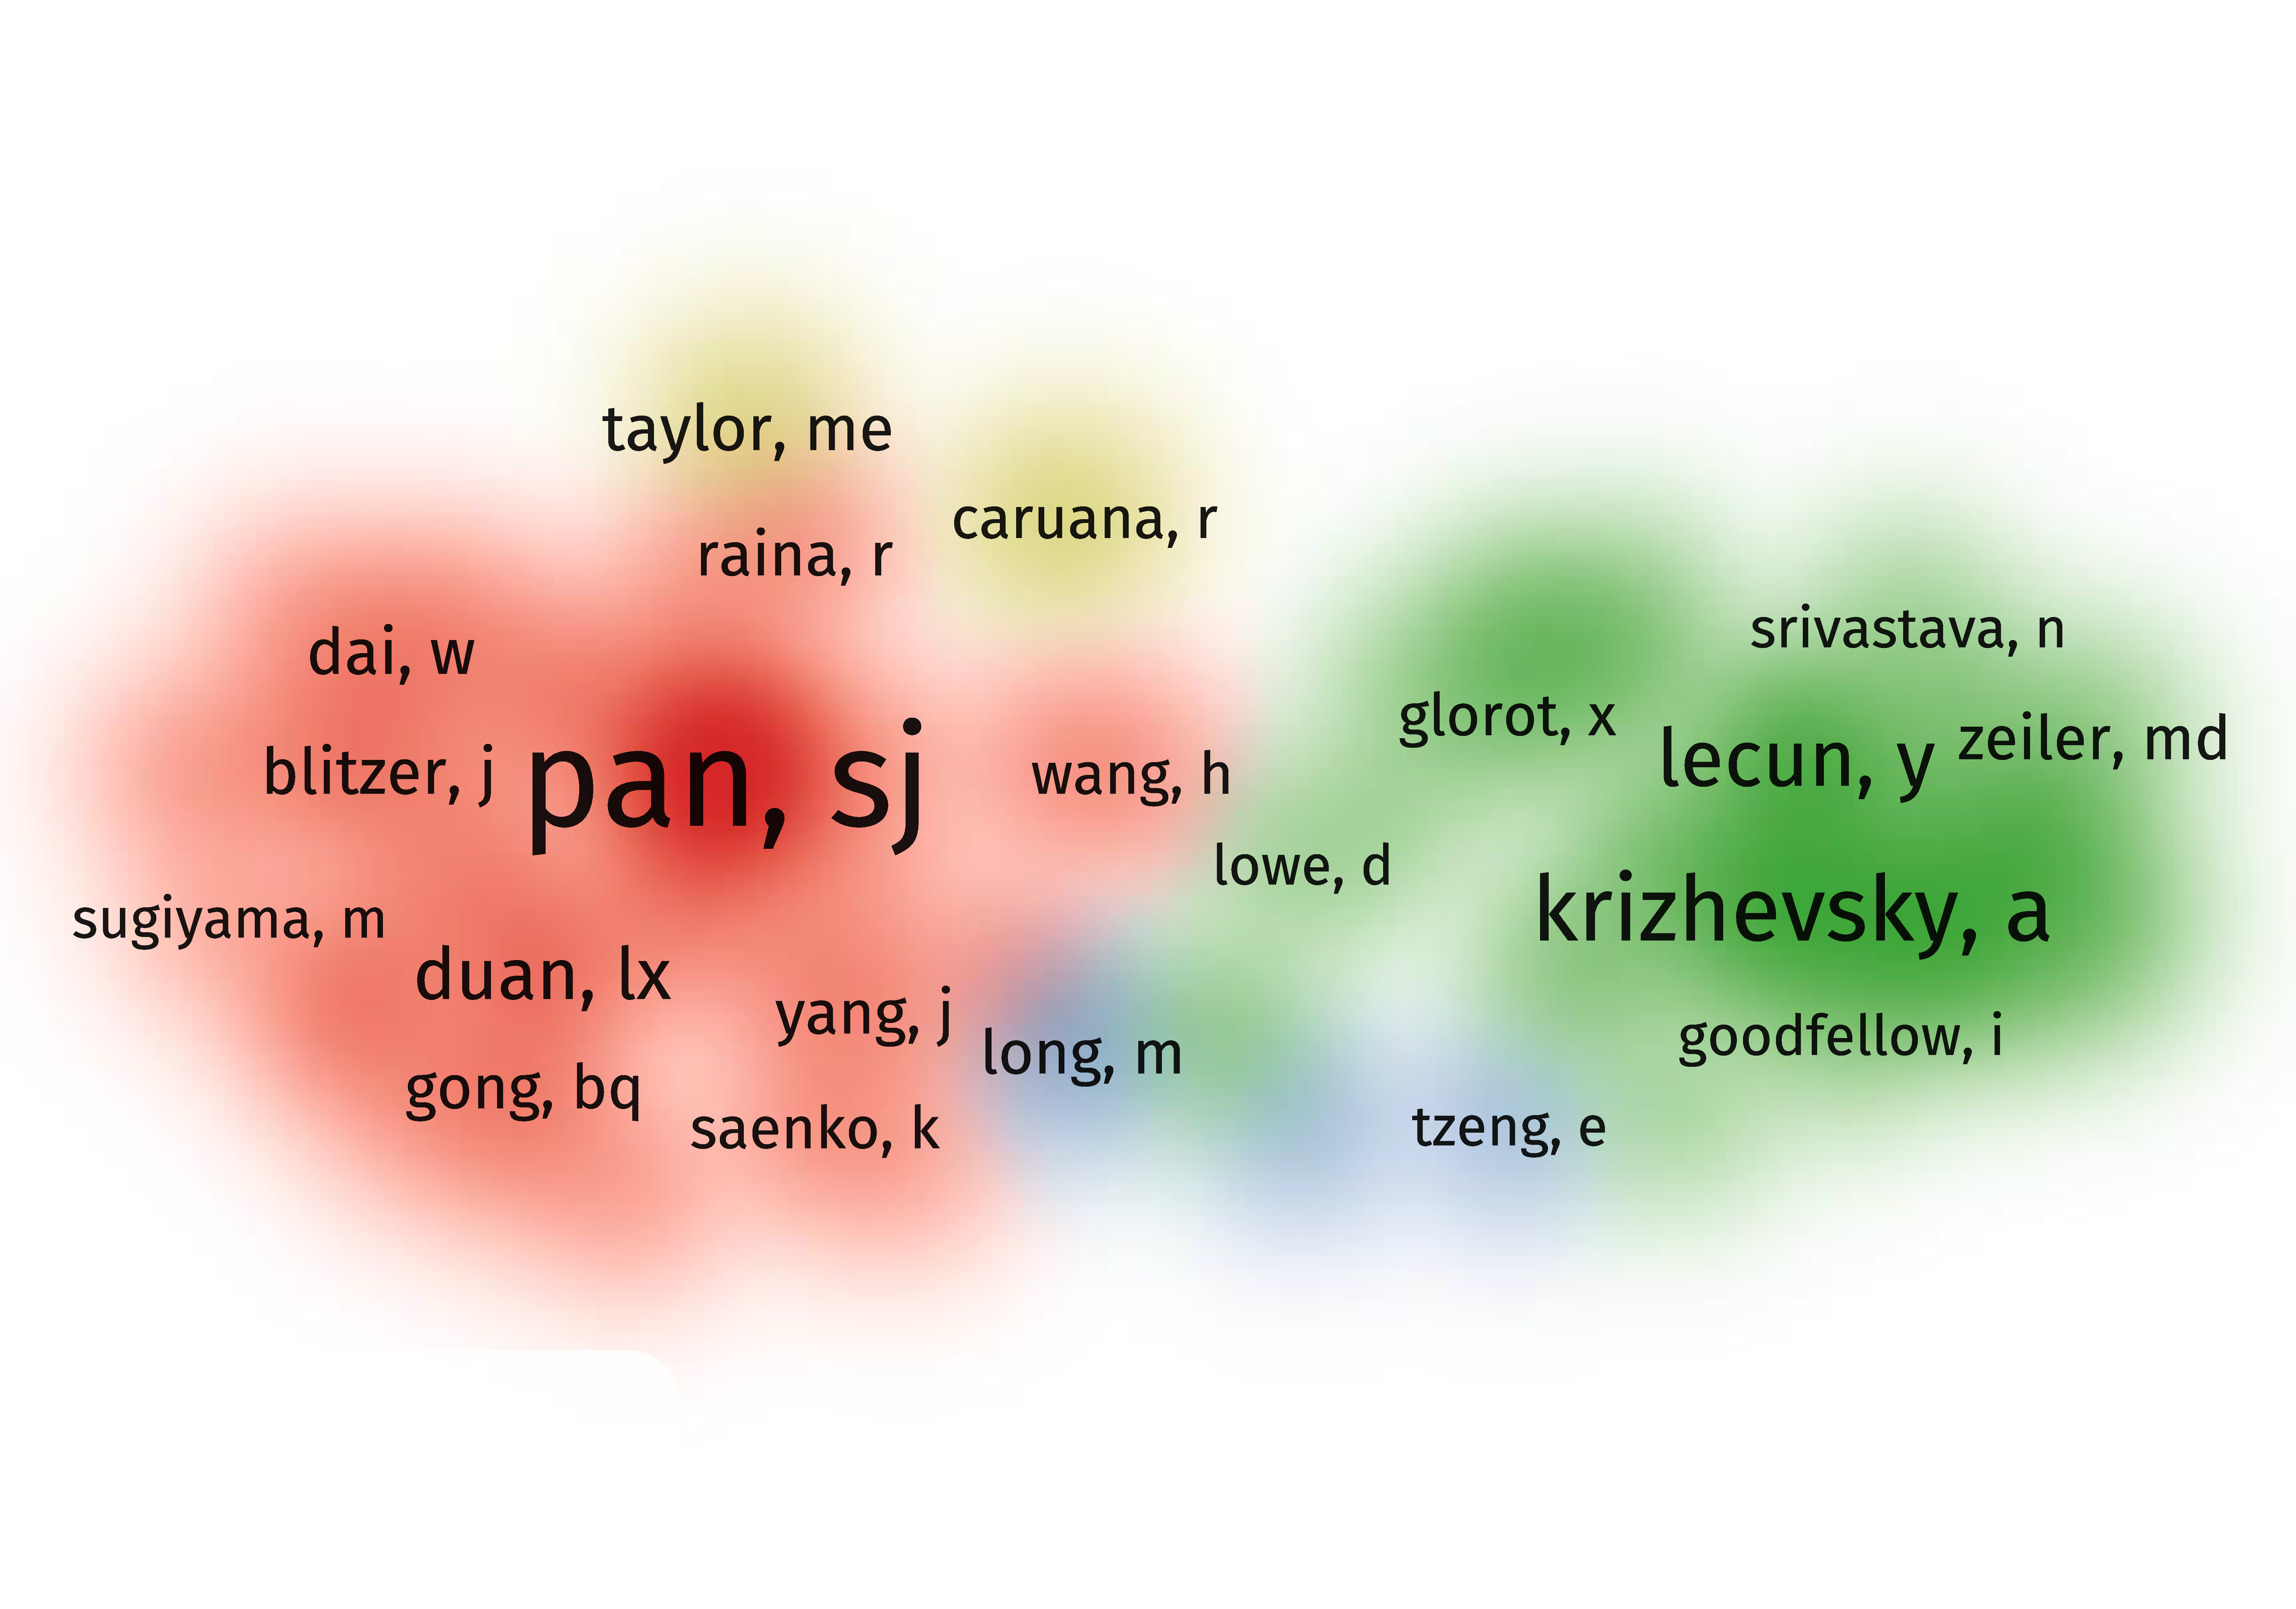
\includegraphics[width=\columnwidth]{completo-4clusters}}
    \source{Dados}{Web of Science (março/2019)}
    \caption{Núcleos de conhecimento obtidos pela análise de co-citações. Os diferentes grupos representam autores que normalmente são co-citados nos 1268 artigos resultantes da busca realizada.}
    \label{fig:classicos}
  \end{figure}
  

 
  \subsection{Os Clássicos}
  \begin{figure*}[b]
    \centering
    \fbox{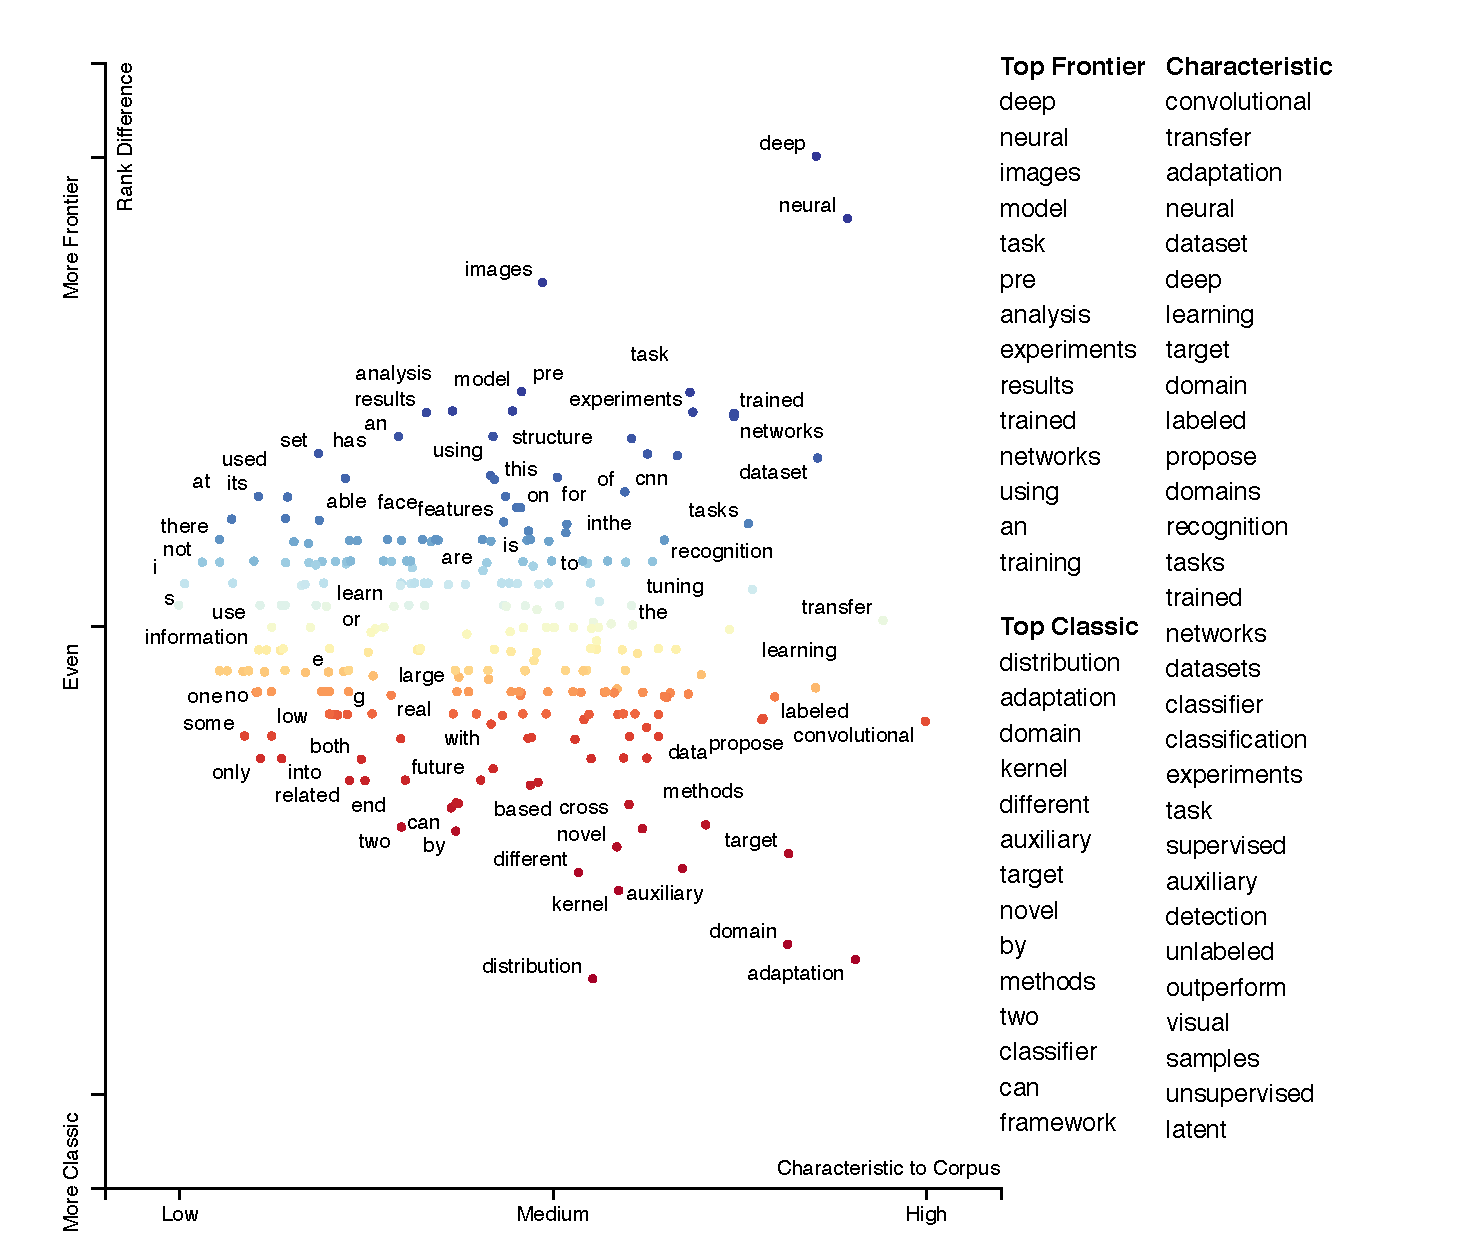
\includegraphics[width=\dimexpr \textwidth-2\fboxsep-2\fboxrule\relax, height= 12cm]{Frontier.pdf}}
    \caption{} \label{fig:studysite}
  \end{figure*}

  \lipsum[3]
  \begin{figure}[t]
    \fbox{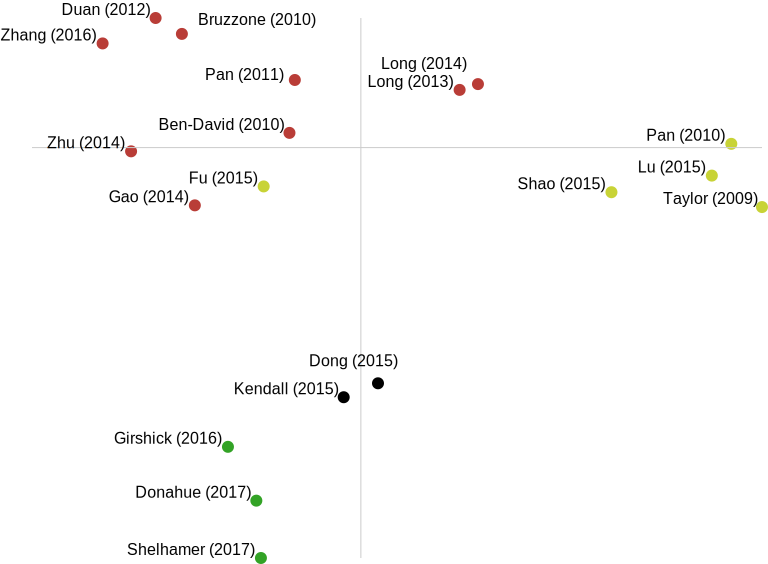
\includegraphics[width=.9\columnwidth]{top20_scatter.pdf}}
    \caption{} \label{fig:studysite}
  \end{figure}
  
  \subsection{A Fronteira}
  \lipsum[2]
  

\section{Problemas em Aberto}
\lipsum[3]
\section{Conclusão}
\lipsum[3]
\bibliographystyle{ACM-Reference-Format}
\bibliography{references}
\end{document}
